\chapter{Experimental Evaluation}\label{chapter:experiments}
In this section we describe the experimental environment and provide details about the criteria we chose to focus on, and the steps followed in our experiments. Besides that, we discuss the corresponding results. The project's source code and other supplementary material are available on GitHub\footnote{\url{https://github.com/perikost/master-thesis}}.

\section{Experimental Setup}\label{sec:}
\subsection{Local experiments}\label{sec:}
We conducted our experiments on a machine with i7-8700 CPU, 64GB RAM, 2TB SSD running Ubuntu 20.04. All SCs were written and compiled in Solidity 0.8.12 with the optimizer disabled and were deployed on Ropsten Testnet. Geth version 1.10.16 was used as an Ethereum client. For IPFS and Swarm, IPFS-client version 0.7.0 and Swarm Bee Client version 0.5.0 were used, respectively.
\subsection{Remote Experiments}\label{sec:setup_remote}
We utilized Grid5000 \citep{bolze_2006}, a robust and versatile platform, for the evaluation of IPFS and Swarm regarding remote retrieval performance. 

Grid5000 is designed to support experiment-driven research in the fields of computer science and networking.
% a wide variety of research areas including parallel and distributed systems, networking, and cloud computing among others.
 The grid's infrastructure consists of around 15,000 cores and 800 compute-nodes spread across different sites in France and organized in clusters. It offers a highly controllable computing environment, allowing researchers to run complex experiments on a large scale. These features allowed us to simulate a real-world environment of nodes spread across different geographic regions to thoroughly test the performance of IPFS and Swarm.
% , and each site hosts clusters of high-performance computing nodes.

% Grid'5000, specializing in computer science research, particularly excels in the realm of parallel and distributed computing, which includes areas like Cloud, High Performance Computing (HPC), Big Data, and Artificial Intelligence (AI).
\begin{table}[H]
\centering
\begin{small}
\caption{Grid5000's sites and clusters we utilized to conduct our experiments.}
\label{tab:grid500}
\resizebox{\textwidth}{!}{%
\begin{tabular}{@{}lcccccc@{}}
\toprule
Site & Cluster & Nodes & CPU & Memory & Storage & Network \\ \midrule
Grenoble & dahu & 32 &  16 cores/CPU & 192 GiB & 720 GB SSD & 10 Gbps + 100 Gbps Omni-Path \\
& & &  & & + 4.0 TB HDD & \\
Lille & chetemi & 14 & 10 cores/CPU & 256 GiB & 600 GB HDD & 2 x 10 Gbps (SR‑IOV)  \\
Nancy & graphite & 4 & 8 cores/CPU & 256 GiB & 600 GB SSD & 10 Gbps (SR‑IOV) + 56 Gbps InfiniBand \\
Rennes & paravance & 72 & 8 cores/CPU & 128 GiB & 1.2 TB HDD & 	2 x 10 Gbps (SR‑IOV) \\
Sophia & uvb & 30 & 16 cores/CPU & 96 GiB & 250 GB HDD & 1 Gbps (SR‑IOV) + 40 Gbps InfiniBand  \\
\bottomrule
\end{tabular}
}
\end{small}
\end{table}



Our experimental topology consists of twelve nodes in total, six for IPFS and six for swarm, which were installed in different geographic regions and participated in the respective public networks. Five IPFS and five Swarm nodes were installed in different regions of france on the Grid5000 platform. A distinct site was chosen to set up each node. Table \ref{tab:grid500} provides an overview of the hardware specifications and the geographic region of each site. Additionally, we utilized our machine (degroot), which based in the city of Xanthi in Greece, to host another two nodes. The clients we installed are IPFS Go client v0.16.0 and Bee client v1.16.0.

We used these controlled instances to interact with the public networks of IPFS and Swarm and perform performance-centric experiments. In order to accomplish this, we developed the necessary code-base for coordinating the nodes. Briefly, in every experiment one machine acts as a server that sends instructions to the remaining machines (clients). The clients respond to each instruction accordingly and forward the results back to the server. In our setup, degroot acts both as a client and a server. 

The experiments have a circular flow with x = 6 rounds, where x signifies the number of nodes that participate in each network. Upon each iteration, a node uploads data of varying sizes and broadcasts the resulting content identifiers to the server. The server, in turn, promts the rest of the nodes (clients) to download the data. Each client keeps track of the time it took for the data to arrive and relays the results back to the server. To account for failures due to retrieval timeouts, our code is designed to allow for retries. 
\section{Criteria}\label{sec:}
For evaluating the sustainability of using Ethereum as a stand-alone data store, we emphasized on the associated gas cost. In this regard, we thoroughly examined the most common storage methods, the SC storage, and the event-logs. Considering these as reference points, we explored alternatives and cost-wise compared the resulting gas costs. In addition, the implementation complexity of each approach was considered. Our findings are summarized in Table~\ref{table:overall}. Among others, the results confirm that the use of SC storage incurs costs that are orders of magnitude larger than the alternative data stores we examined.

Except for being monetarily viable, DApps need to perform adequately when it comes to retrieving data. That being said, we measured the retrieval time in all the above scenarios. For IPFS and Swarm, both local and remote latency were taken into account, aiming to a better overall comparison.
\section{Storing Data in Ethereum}\label{sec:evaluation_ethereum}
Before proceeding further, we should mention an important detail concerning the data we used during our experiments. Solidity uses UTF8 encoding, according to which common ASCII characters are represented by a single byte. Additionally, generating random fixed-length character sequences is simple and all the methods we examined support this format. So, to evaluate the cost of storage in Ethereum, for each test case, we recorded 15 measurements regarding various string sizes equally spread across the range of 1B-16KB. For those cases that exhibit consistent behavior we present only part of our measurements.

\subsection{SC Storage}\label{subsection:evaluation_sc}
\begin{figure}[htbp]
    \begin{subfigure}{\linewidth}
        \centerline{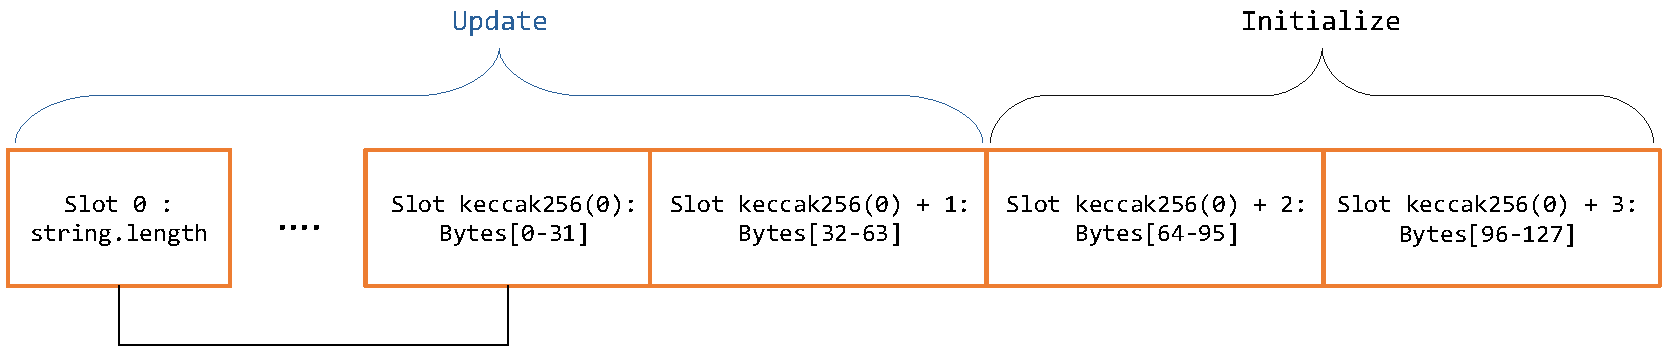
\includegraphics[width=\textwidth]{figs/Storage1.pdf}}
        \caption{}
        \label{fig:arrays_1}
    \end{subfigure}
    \begin{subfigure}{\linewidth}
        \centerline{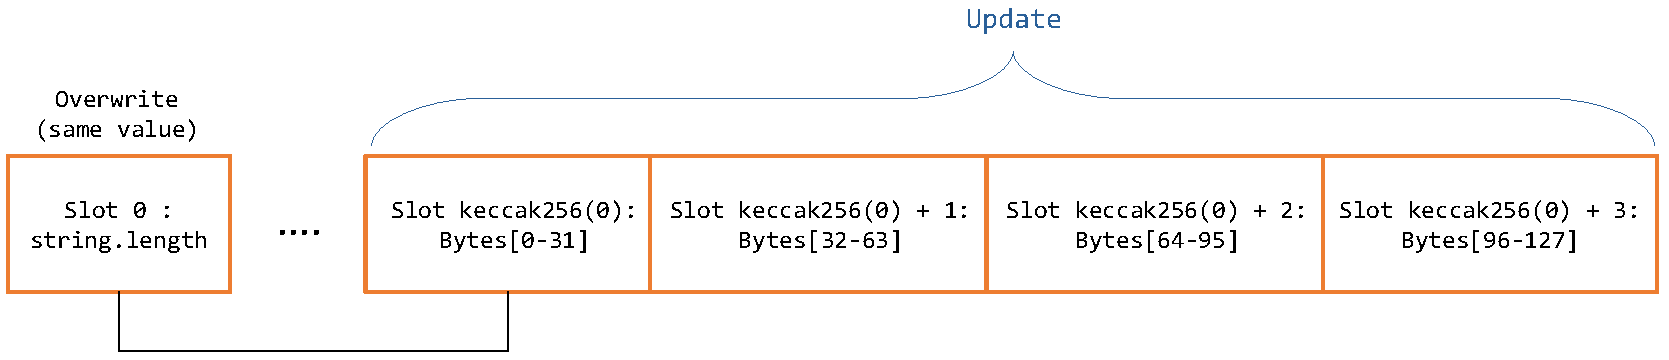
\includegraphics[width=\textwidth]{figs/Storage2.pdf}}
        \caption{}
        \label{fig:arrays_2}
    \end{subfigure}
    \caption{Slots that must updated or initialized when overwriting a string with (a) a longer (b) a new one of the same size.}
\end{figure}

In order to perform this experiment, we designed a simple SC with the following elements: a public string variable to store our data, a function to modify this string and another one to reset it. In total, we tested three of the most common scenarios.

% TODO: maybe with instead of to?
\begin{itemize}[topsep=0pt, itemsep=0pt]
  \item Storing data after resetting the variable (clean storage).
  \item Updating the variable to a longer string (double the size), Fig.~\ref{fig:arrays_1}.
  \item Updating the variable to a new string (same size), Fig.~\ref{fig:arrays_2}.
\end{itemize}

The baseline of 21000 gas for every transaction and the gas paid for its payload are equal in all three cases. So, the number of slots that must be overwritten or initialized during each test case mostly accounts for the difference in the respective costs depicted in Fig.~\ref{fig:store1} and Fig.~\ref{fig:store2}, which was included to present the costs for small data. For data less than 32 bytes, as discussed in subsection~\ref{sec:sc_storage}, one slot is adequate. Otherwise, \(\ceil*{x/32}\) slots for storing the data and one for storing the string's size \(x\), are required. In the case of clean storage, all slots must be initialized, costing \(20000*num\_slots\) gas. When updating a string with a new one of the same size, 5000 gas is deducted for each of the \(\ceil*{x/32}\) slots. Note that the slot holding the string’s length is not updated, as the string’s size does not change. In fact it is overwritten with the same value, which is termed as a \emph{``no-op''} and is charged equally to an SLOAD operation. The second case is a combination of the others and so is the cost calculation method. Some slots must be initialized, and others need to be updated, costing 20000 and 5000 each.

\begin{figure}[htbp]
\centerline{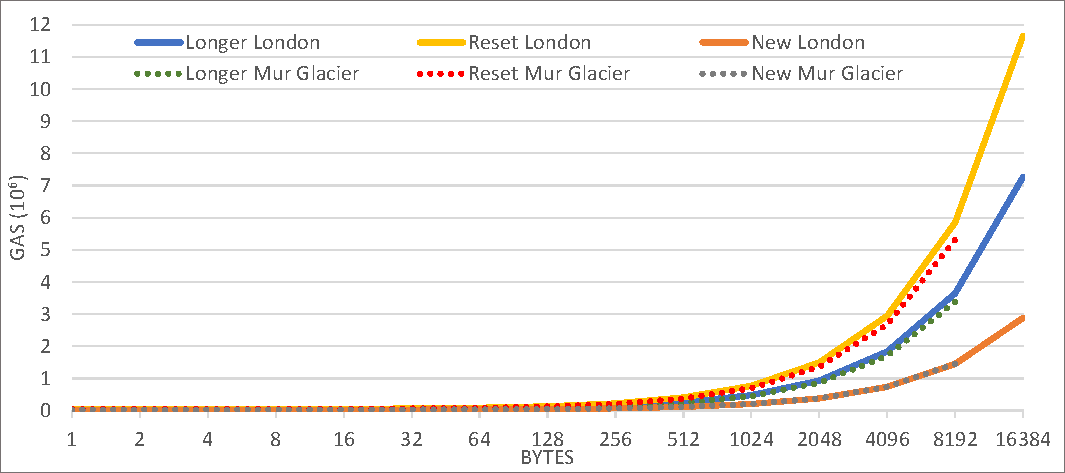
\includegraphics[width=\textwidth]{figs/store1.pdf}}
\caption{SC storage cost diagram.}
\label{fig:store1}
\end{figure}

\begin{figure}[htbp]
\centerline{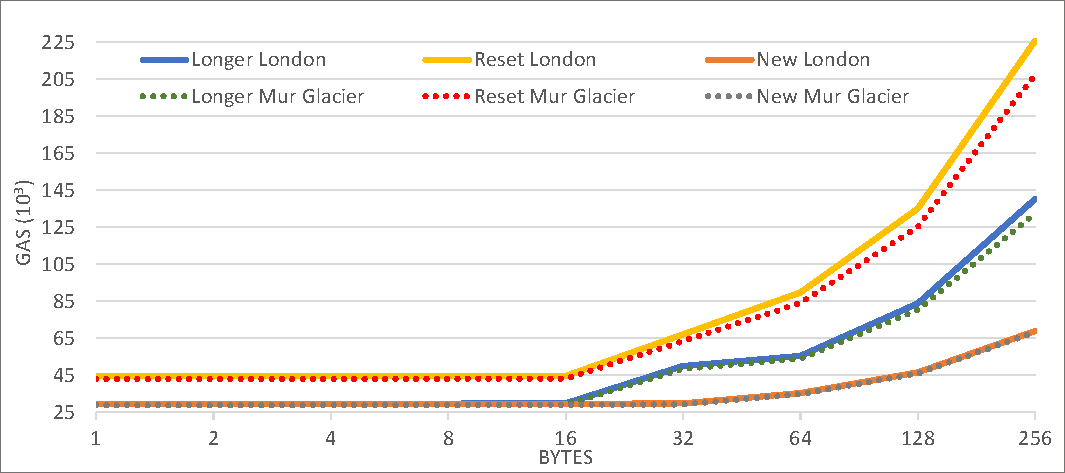
\includegraphics[width=\textwidth]{figs/store2.pdf}}
\caption{Zoomed in view of the diagram in Fig.~\ref{fig:store1}.}
\label{fig:store2}
\end{figure}

Up to this point, we discussed gas consumption based on the EIPs introduced prior to (including) Muir Glacier. EIP-2929, included in Berlin fork, reforms SLOAD and SSTORE gas metering.

% TODO: cite EIP-1559
Considering the altered cost model outlined in paragraph \ref{par:eip_2929_cold_warm}, we re-executed all test cases to examine Ethereum’s actual behavior after the Berlin hard fork. In order to be up-to-date, we also repeated our study when the London hard fork was implemented. Gas consumption related to the SSTORE and SLOAD operations was not altered by any of the included EIPs. However, EIP-1559 specifies a transaction pricing mechanism that temporarily raises the block’s gas limit when congestion occurs. This enabled us to store up to 16KBs in contrast to the 12KBs that we managed to store in previous experiments. In Fig.~\ref{fig:store1} we present our most recent results, since they reflect the impact that both hard forks induced.

Overall, all transactions after EIP-2929 had a higher cost, especially those regarding our first test case, in which, every slot had to be initialized imposing an overhead of 2100 gas. Regarding the third test case, all transactions executed after the fork proved to cost 600 more. By debugging those, we discovered that this difference is caused by the SLOAD gas metering modification. Basically, when updating a string, the slot that holds the string’s length is accessed twice; once to determine the string’s length (SLOAD) and a second time to update it to the new length (SSTORE). The SLOAD operation is considered a COLD\_SLOAD and costs 2100 gas. The SSTORE on the currently \emph{``warm''} slot is considered a \emph{``no-op''} since the length of the string remains the same and costs 100 gas. Before EIP-2929 took effect, these operations were charged 800 each.

\begin{figure}[htbp]
\centerline{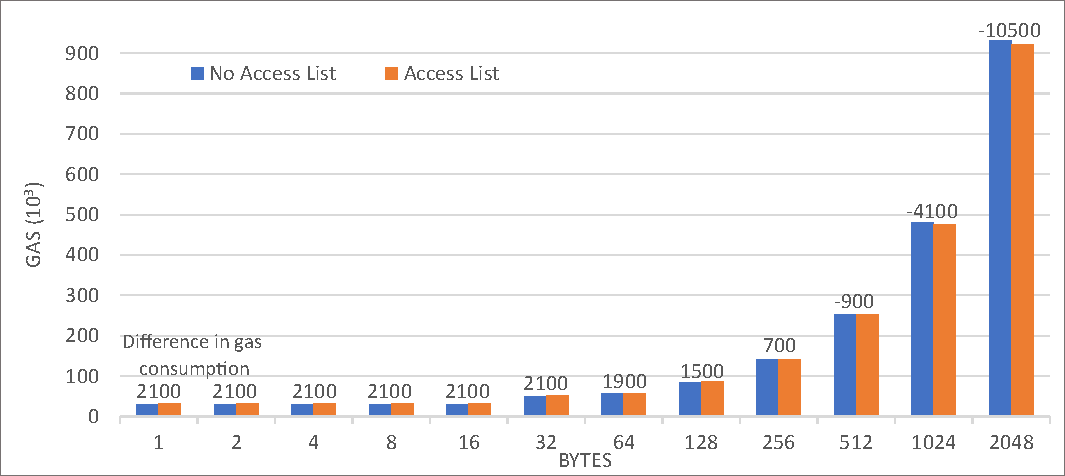
\includegraphics[width=\textwidth]{figs/access_list.pdf}}
\caption{SC storage cost diagram (optional AL).}
\label{fig:access_list}
\end{figure}

Besides EIP-2929, EIP-2930 was also included in the Berlin hard fork. As a result, users can now specify a list of addresses and storage keys that the transaction plans to access, which are \emph{``warmed up''} and consequently subsequent accesses come at a discounted price (see paragraph \ref{par:eip_2930_access_list}).

Based on Table~\ref{table:access_list} one would assume that declaring an AL is a better option, at all times, as 100 gas would be saved for every account/storage access and 200 gas for every SSTORE operation. However, that is not the case. If storage keys of the targeted contract are specified in an AL, the targeted contract account must be included as well, imposing an overhead of 2400 gas.
% TODO: add https://eips.ethereum.org/EIPS/eip-3521

\begin{figure}[htbp]
\centerline{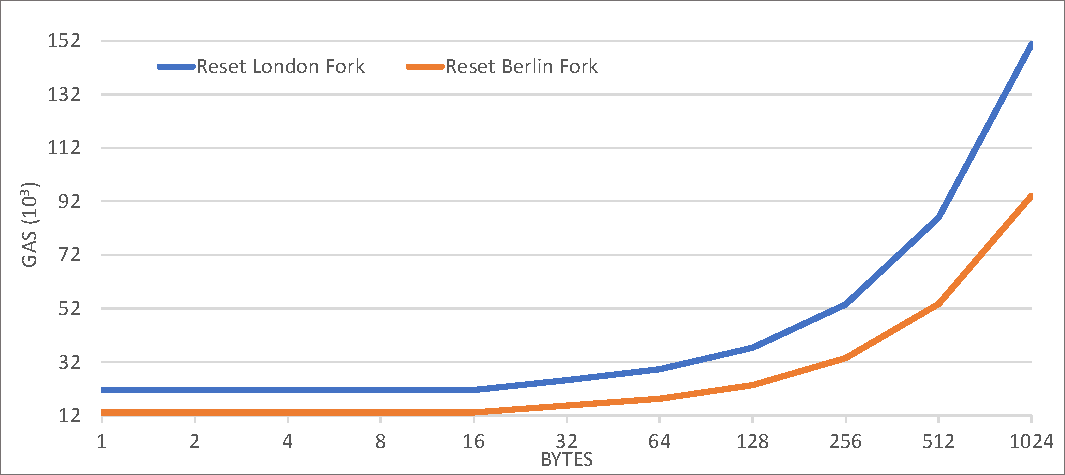
\includegraphics[width=\textwidth]{figs/reset.pdf}}
\caption{Cost of clearing SC storage.}
\label{fig:reset}
\end{figure}

The behavior described above is depicted in Fig.~\ref{fig:access_list}. When the string’s size is under 352 bytes, using an AL is more expensive due to the gas paid for including the contract’s address. On the contrary, storing a string longer than 352 bytes is more cost-efficient if an AL is declared. In brief, the 2400 overhead is countered by the 12 or more SSTORE operations that access each of the storage slots that contain the string's data and the SLOAD operation required to determine the string's length, which are charged at a discounted rate, i.e., 200 and 100 less gas respectively.

% TODO: if one uses access list they should refrain
As a general guide, one should opt in for the use of ALs, but refrain from specifying storage slots of the targeted contract account. Yet, if the main contract interacts with other contracts, which then access their storage, specifying their addresses (but not tx.to) and storage keys in an AL is less expensive than not using an AL.

Handling the data of a DApp involves data storage, retrieval and deletion. In Ethereum, SC storage is considered a valuable resource and therefore a gas refund is given when data is erased.

In Fig.~\ref{fig:reset}, we present the overall cost associated with clearing the slots occupied by a string’s data. Considering that clearing a slot entails updating its value from non-zero to zero, the actual execution cost is comparable to that of updating a string to a new one (see Fig.~\ref{fig:arrays_2}), except that in this case the string's length is also updated; 5000 gas is charged for every SSTORE operation on the slots that the string occupies. Though, the refund granted for these operations contributes to a lower overall transaction cost.

London hard fork introduced EIP-3529  \citep{buterin_eip_3529} which modified the refund mechanism (see paragraph \ref{par:eip_3529_refund}). Prior to this, emptying a slot was rewarded with 15000 gas and the total refund was capped at 50\% of the transaction’s gas used. In the London fork implementation both the reward and the refund were reduced to 4800 gas and 20\%, respectively. Fig.~\ref{fig:reset} demonstrates the impact that this modification has on the cost related to deleting a string. All transactions incurred an increase of approximately 38\% in gas usage.

\subsection{Event-logs}\label{subsection:evaluation_logs}

Prior to any further analysis, we ought to mention that in preliminary experiments \citep{kostamis_2021}, counters were used as identifiers (ids) for the events, as illustrated in Table~\ref{table:event}. However, the use of counters entails the execution of an SLOAD operation, which gets their values in order to pass them as parameters to the events and also an SLOAD and SSTORE operation for incrementing them, imposing an overhead of 6600 gas in every transaction. Considering this, we decided to re-execute the experiments and pass the ids as arguments. Hence, the results presented in this work are rather indicative of the effect that emitting an event has on gas consumption, as the need for extra contract logic was eliminated.

As we can observe in Fig.~\ref{fig:logs} the resulting costs from calling each event, exhibit relatively small divergence. Through  \citep{wood_2014} we know that each topic costs 375 gas. Respectively, there is a charge of 8 gas for each byte of data recorded in the data field of the logs. Thereby, the number of topics generated by the event call in each of the cases we examined, as well as the amount of data recorded in the log data field, are key factors in the cost variance between them. These are determined by the way the events are declared, as shown in Table~\ref{table:event}. If the id is indexed it is placed in the topics array along with the event’s signature hash, otherwise it is ABI encoded into the data field of the log. Additionally, since the input data are identical in all the events and the contract's code is immutable by default, the constant gap maintained by the four graphs is justified.

\begin{table*}[]
\caption{Structure of events and logs included in the experiments}
\centering
\label{table:event}
\resizebox{15cm}{!}{%
\begin{tabular}{@{}ccccc@{}}
\toprule
 & \textbf{Indexed} & \textbf{Non-Indexed} & \textbf{Anonymous Indexed} & \textbf{Anonymous} \\ \midrule
\textbf{Declaration} & \begin{tabular}[c]{@{}c@{}}event\_name(uint indexed id, \\ string data)\end{tabular} & \begin{tabular}[c]{@{}c@{}}event\_name(uint id, \\ string data)\end{tabular} & \begin{tabular}[c]{@{}c@{}}event\_name(uint indexed id, \\ string data) anonymous\end{tabular} & \begin{tabular}[c]{@{}c@{}}event\_name(uint id, \\ string data) anonymous\end{tabular} \\
\textbf{Topic{[}0{]}} & keccak(event\_signature) & keccak(event\_signature) & - & -\\
\textbf{Topic{[}1{]}} & abi\_encode(id) & - & abi\_encode(id) & - \\
\textbf{Log Data} & abi\_encode(data) & abi\_encode(id, data) & abi\_encode(data) & abi\_encode(id, data) \\ \bottomrule
\end{tabular}%
}
\end{table*}

It should be noted that because log data is ABI encoded, even a uint8 occupies 32B and is charged \( 8*32 = 256 \) gas. For this reason, converting a non-indexed parameter to an indexed does not impose much of an overhead. In fact, it is negligible since the opcodes that are executed to determine the function to be called, might result in the indexed event being less expensive. That is the case for the anonymous events, as indicated in Fig.~\ref{fig:logs}.

Finally, even though anonymous events are the least expensive option, they should be used frugally. The fact that they don’t register their signature as a topic, prohibits them from being uniquely referenced, perplexing their retrieval. Including indexed parameters to such events can assist with that.

% Finally, it is apparent that the use of SC storage incurs costs that are orders of magnitude larger than the currently discussed alternative.

\begin{figure}[htbp]
\centerline{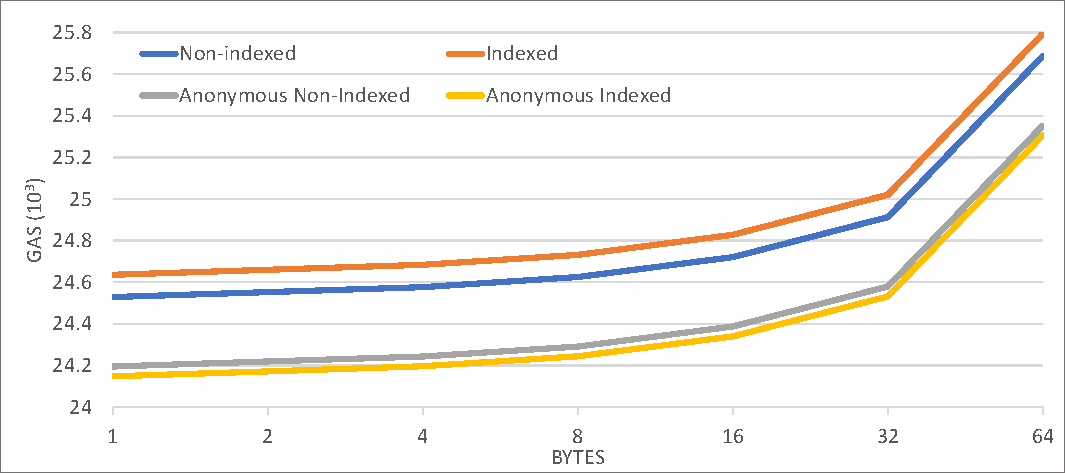
\includegraphics[width=\textwidth]{figs/logs_1.pdf}}
\caption{Event-logs storage cost diagram.}
\label{fig:logs}
\end{figure}

\subsection{Transaction Payload}\label{subsection:evaluation_payload}
The first step of this experiment was to encode the data in hex format. Then, we included the resulting hex byte array in the data field of a transaction object, signed it and sent it. Note that no ether was transferred during any of the transactions. We tried two different ways of implementing this method:

\begin{itemize}[topsep=0pt, itemsep=0pt]
  \item Sending the transaction between EOAs
  \item Sending the transaction from an EOA to a CA
\end{itemize}

As expected, the measurements confirm that the use of transactions as a data store is the most cost-efficient solution of all when data is sent between EOAs. As a matter of fact, this can be considered the minimum cost for storing data in Ethereum. That is, because the fee paid for a transaction’s payload is essentially included in every available option, e.g., for executing a transaction with some data as input, these data must first be sent as payload to the contract.

For the second case we tested, a fallback function in the targeted SC is required, otherwise the transactions will fail. In short, fallback is a special function that gets executed if none of the function selectors match the first four bytes of the transaction payload, or if the latter is empty and no Receive Ether function is defined. Additionally, it cannot have parameters nor return anything. The body of the fallback could either be empty or include function logic. In any case, if arbitrary hex-encoded data is included in the payload of a transaction that is targeted to a SC, the fallback will be executed (no function selector will be matched) and the data will be permanently saved in the blockchain, as part of the transaction. Implementing an empty fallback entails that the transaction hash must be saved externally. On the contrary, emitting an event inside the fallback allows the user to obtain the transaction hash from the resulting logs and retrieve the data from the recorded transaction.

\begin{figure}[htbp]
\centerline{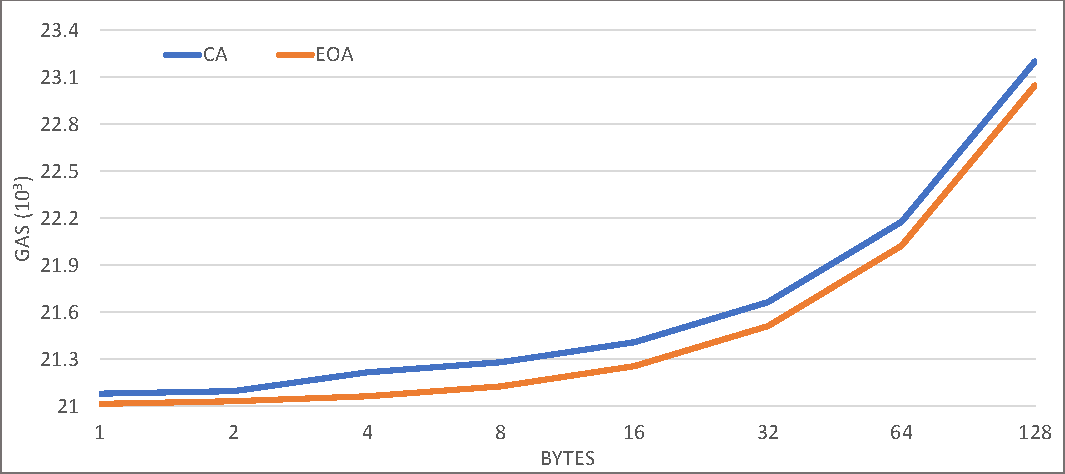
\includegraphics[width=\textwidth]{figs/tx.pdf}}
\caption{Transaction payload storage cost diagram.}
\label{fig:tx}
\end{figure}

Based on Fig.~\ref{fig:tx}, we are able to compare the cost of saving data in a transaction payload that is sent to an EOA or a CA, respectively. Regarding the latter scenario, the SC implements an empty fallback function. The difference between the amount of gas spent in each test case stems from the fact that in the second one some contract code needs to be executed. By inspecting the bytecode of the corresponding contract, we managed to further analyze this difference. After verifying that no ether was sent with the transaction, a series of opcodes is executed to check if the payload is less than four bytes. If that is true, EVM jumps to fallback’s execution. The accumulated cost resulting from the EVM execution, up to that point, is 65 gas greater than that of test Case 1. If the aforementioned condition is false, the first four bytes of the payload are loaded and processed, costing 12 gas, and they are compared against every function selector of our contract’s three functions. Eventually, no match is found and the execution jumps to the fallback function, which costs 10 gas. The code blocks in which the comparisons are conducted consist of the opcodes \textsc{\{dup1, push4, eq, push2, *jumpi\}}, which altogether cost 22 gas. Taking into account that no match will be found, all comparisons are executed, costing 66. In total, the cost for storing \(data\geqslant 4\) bytes in a transaction by exploiting the fallback function, is 153 gas greater than the other test case.


By inspecting the execution of the contract at bytecode level we managed to verify what to our knowledge was first reported, but not explained, in \citep{chen_2018}. Simply put, function selectors, which are comprised of the first four bytes of the Keccak-256 hash of the function's signature and therefore depend on function names and parameter types, are compared to the first four bytes of a transaction’s payload in hex-ascending order. Hence, frequently used functions should be named in an appropriate manner to avoid numerous comparisons, i.e., save gas. Moreover, we believe it is necessary to point out that for a contract with a large number of functions, Solidity optimizes the comparison flow by performing a pre-comparison to check whether the given function selector is or is not above a certain threshold.

As already mentioned, an event could be emitted inside the fallback function to avoid saving the transaction hash off-chain. Similarly to the experiments in~\ref{subsection:evaluation_logs}, the event should include an id parameter so that the data can be identified upon retrieval. This was achieved in two ways: i) increasing a counter in every call ii) reserving some bytes of the transaction data (e.g., the first 32bytes) to hold the id. The latter is generic since values other than integers can be used, but requires additional logic, both on-chain and off-chain, to separate or concatenate the data and the id. In addition, eschewing the use of a counter significantly reduces the gas consumption, as depicted in Fig.~\ref{fig:fallback}. In fact, since the cost of the log operation is identical in both cases, the difference in the cost depends solely on the need of updating the counter, which involves two SLOAD and one SSTORE operations.

\begin{figure}[htbp]
\centerline{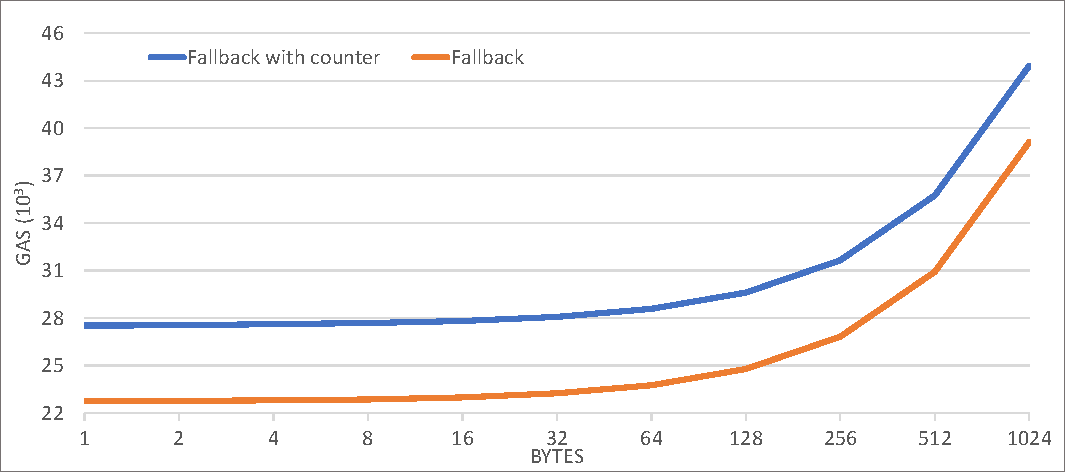
\includegraphics[width=\textwidth]{figs/fallback.pdf}}
\caption{Cost of emitting an event inside the fallback function.}
\label{fig:fallback}
\end{figure}

\subsection{Unused Function Parameters}\label{subsection:evaluation_unused}
This experiment was performed to examine the cost of storing data in a transaction’s payload while exploiting Solidity’s built-in ABI interface.
Such a scheme overcomes the restriction imposed by the previous method as it facilitates the management of all the data types that Solidity supports, without the need of additional client logic. 

% we used a function with a single parameter that was no further processed.
% \hl{We also decided to improve the functionality of this method by emitting an event, with just one indexed parameter, inside the function in order to track the hash of the transaction at a later point}.
In order to examine this approach, we declared a function with two parameters; one to hold the data and another one to hold an identifier. The former was no further processed, while the latter was passed to an event. Emitting an event inside the function enabled us to obtain the transaction hash from the resulting logs and retrieve the ABI encoded data from the recorded transaction. In contrast to the utilization of a fallback function, which cannot accept any arguments, the id of the event is passed as a function argument eliminating the need for additional contract logic.

To evaluate the recorded costs, we used the case of indexed events as a reference point. It is obvious from Fig.~\ref{fig:unused} that as input data grow in size, the current approach gets even cheaper than the other. The fact that in this case, no data are recorded in the data part of the produced log, accounts for the difference.

\begin{figure}[htbp]
\centerline{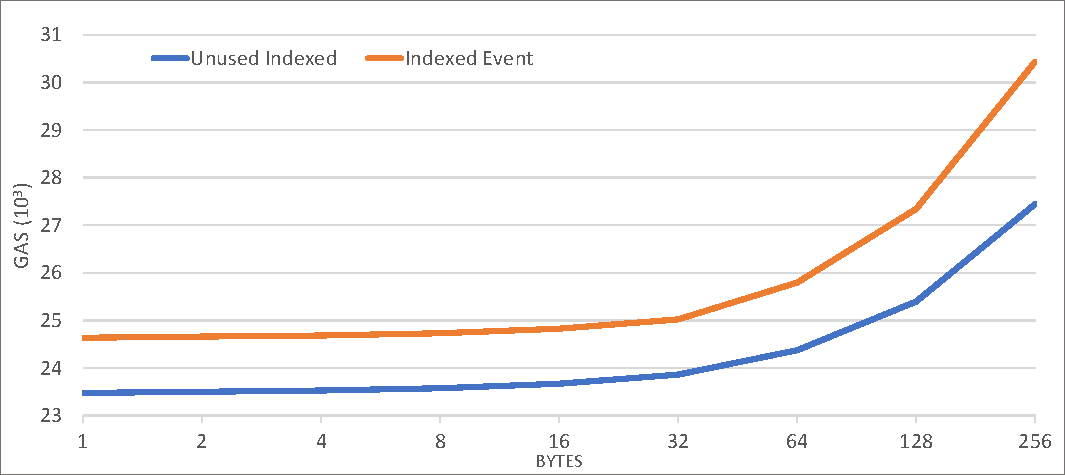
\includegraphics[width=\textwidth]{figs/unused.pdf}}
\caption{Unused function parameter and event-logs storage cost diagram.}
\label{fig:unused}
\end{figure}

As we already mentioned, the fact that non-indexed parameters are ABI encoded into the log data leads to long log arrays. So, in a scenario in which more unused parameters are utilized, the current approach is even less expensive. To confirm this, we conducted a complementary experiment, locally in Ganache. A contract with two functions carrying seven parameters each was deployed. Function 1 emitted an event with all parameters as input, whereas Function 2 emitted an event with just the first parameter. After executing both functions with the same arguments, we concluded that the utilization of unused function parameters can be quite effective, as Function 2 cost nearly 7000 less gas.

At this point, we would like to discuss some possible drawbacks regarding this alternative storage method. First, by testing we discovered that Solidity imposes a restriction on the number of parameters a function can bear (around sixteen). If this threshold is exceeded, a \emph{``stack too deep''} error is thrown. Additionally, defining a function with unused function parameters causes a warning at compilation. Thus, it might be disallowed in future Solidity versions.

\section{Data Retrieval in Ethereum}\label{sec:evaluation_ethereum_retrieval}
In this subsection, based on our experimental measurements, we present an overall comparison of the time needed to retrieve data from the Ethereum blockchain. Each measurement refers to the retrieval time of the data that were stored during the previous experiments. We noticed that the results were quite similar for the different data sizes (1B – 16KB), so, in Table~\ref{tab:retrieve} we recorded the average of these results. Also, we should mention that retrieving data stored in unused function parameters is a two-step process: the respective logs must be retrieved to acquire the transaction hash and then the transaction itself must be retrieved to acquire the targeted data. Likewise, using events without indexed parameters implies that additional logic should be implemented to find the desired data among the returned events. In any case, these delays were found to be insignificant compared to the time needed to retrieve the respective events. Thus, all measurements presented in Table~\ref{tab:retrieve} include any necessary additional step.

Considering the measurements presented in Table~\ref{tab:retrieve}, it is obvious that both retrieving data from contract’s storage or retrieving a transaction and extracting its data, require substantially less time than that of the other test cases. That is because these particular retrieval processes are ultimately single database queries that target either the Storage Trie or a Transaction Trie. 

\begin{table}[]
\caption{Retrieval latency in Ethereum (ms)}
\label{tab:retrieve}
\centering
\resizebox{12cm}{!}{%
\begin{tabular}{@{}ccc@{}}
\toprule
 & \multicolumn{2}{c}{\textbf{Retrieval Latency}} \\ \midrule
\textbf{Storage}&\multicolumn{2}{c}{0.89}\\
\textbf{Transaction}&\multicolumn{2}{c}{1.79}\\
\midrule
\textbf{} & \textbf{fromBlock: 0} & \textbf{\begin{tabular}[c]{@{}c@{}}fromBlock: con\_creation\end{tabular}} \\ \midrule
\textbf{Non Indexed Event}&331.33&39.16\\
\textbf{Indexed Event}&276.62&33.04\\
\textbf{Anonymous Event}&1569.76&67.55\\
\textbf{Anonymous Indexed Event}&420.60&36.85\\
\textbf{Unused Inexed Event}&276.44&30.19\\
\textbf{Unused Non Indexed Event}&337.01&34.59\\
\bottomrule
\end{tabular}%
}
\end{table}

On the other hand, the process of retrieving events involves the utilization of BFs and therefore is more complex and leads to higher latency. Though, through an appropriate interface, a developer can specify the block from which the client should start searching for the requested event(s). This can greatly reduce the number of database queries, as less BFs need to be inspected, resulting in faster retrieval. Indeed, we confirmed that searching from the beginning of the blockchain as opposed to specifying a more recent starting point requires significantly more time. In our experiments, as a starting block, we set the ones that our contracts were deployed in since no events could have been emitted before that point. Besides that, we observe that the use of indexed parameters in an event can further improve the retrieval performance.

\begin{figure}
    \begin{subfigure}{\linewidth}
        \centerline{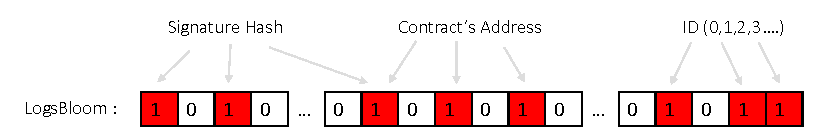
\includegraphics[width=\textwidth]{figs/bloom_indexed.pdf}}
        \caption{}
        \label{fig:bloom_indexed}
    \end{subfigure}
    \begin{subfigure}{\linewidth}
        \centerline{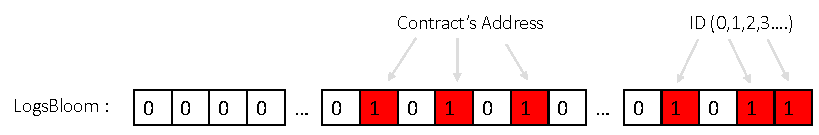
\includegraphics[width=\textwidth]{figs/bloom_anonymous.pdf}}
        \caption{}
        \label{fig:bloom_anonymous}
    \end{subfigure}
    \caption{Example of the bloom bits set by (a) indexed (b) anonymous indexed events.}
    \label{fig:bloom_combined}
\end{figure}

As mentioned in subsection ~\ref{subsection:retrieving_logs}, three bits of the BF are set by the contract’s address and three for every topic. Anonymous events don’t register their signature hash as a topic. Thereby, filtering an anonymous event with no indexed parameters is accomplished by verifying that the three bits that correspond to the contract’s address are set in the BF. However, every event of the same contract would have set these bits as well. In a similar manner, the bits set by the anonymous indexed event we declared, are also set by every other indexed event; given the same uint256 as input for the indexed parameter, the bits they set coincide. The behavior we describe is demonstrated in Fig.~\ref{fig:bloom_combined}. In brief, anonymous events result in a higher false positive rate thus hindering the retrieval process.

\begin{table}[H]
\caption{Retrieval latency in Ethereum with clear cache (ms)}
\label{tab:retrieve_clear}
\centering
\resizebox{12cm}{!}{%
\begin{tabular}{@{}ccc@{}}
\toprule
 & \multicolumn{2}{c}{\textbf{Retrieval Latency}} \\ \midrule
\textbf{Storage}&\multicolumn{2}{c}{1.95}\\
\textbf{Transaction}&\multicolumn{2}{c}{3.98}\\
\midrule
\textbf{} & \textbf{fromBlock: 0} & \textbf{\begin{tabular}[c]{@{}c@{}}fromBlock: con\_creation\end{tabular}} \\ \midrule
\textbf{Non Indexed Event}&1156.90&44.78\\
\textbf{Indexed Event}&1128.71&33.54\\
\textbf{Anonymous Event}&4034.35&78.19\\
\textbf{Anonymous Indexed Event}&1289.72&38.84\\
\textbf{Unused Inexed Event}&1136.50&31.93\\
\textbf{Unused Non Indexed Event}&1154.05&39.29\\
\bottomrule
\end{tabular}%
}
\end{table}

It is noteworthy that Geth uses LevelDB to manage the blockchain's data. Driven by the fact that most operating systems utilize free RAM memory for caching, we decided to assess how the system’s cache may influence the retrieval performance. In short, recently accessed LevelDB files are cached by the OS and therefore subsequent requests are served faster. So, we repeated our experiments but dropped the page cache between each run, as it is proposed in  \citep{perez_2020}, and gathered the measurements in Table~\ref{tab:retrieve_clear}. This dramatically delayed the retrieval of data from logs when the starting block was set to zero (i.e., beginning of the chain). Basically, when filtering from block zero, a lot of LevelDB files are accessed to find a specific log. The fact that these files are loaded from disk when they are not available in the system’s cache, justifies this delay. On the other hand, since the required disk accesses are greatly reduced when the search is conducted with a more recent starting point, the retrieval latency is not affected to the same extent.



\begin{table*}[!htb]
\begin{small}
\centering
\caption{Overall comparison of Ethereum's data stores.}
\label{table:overall}
\resizebox{\textwidth}{!}{%
\begin{tabular}{@{}p{0.14\linewidth}p{0.14\linewidth} p{0.13\linewidth} p{0.13\linewidth} p{0.46\linewidth}@{}}
\toprule
& & \textbf{Storage Cost} & \textbf{Retrieval Latency} & \textbf{Comments} \\
\midrule
\textbf{Storage} & & Very High & Very Low & Viable option only when storing small data. Should host all the data that is essential for the SC's proper operation, since data stored using any of the alternative methods is not accessible within the SC. \\
\midrule
 \textbf{Event-logs} & \textbf{Non-Indexed} & Low & Moderate & \multirow{4}{=}{Suitable for archiving data at a low cost. Filtering specific logs is time consuming but limiting the filtering block-range and exploiting indexed parameters can accelerate the process. Thus, events should be declared according to the DApps' needs, so that high latency is avoided.} \\
 & \textbf{Indexed} & Low & Moderate & \\
 & \textbf{Anonymous} & Low & Very High & \\
 & \textbf{Anonymous Indexed} & Low & High & \\
 \\
 \\
\midrule
\textbf{Transaction Payload} & \textbf{CA} & Very Low - Moderate & Very Low - Very High & \multirow{4}{=}{Least expensive method if the target is an EOA. The transaction hashes must be saved off-chain. In case of transactions to CAs, the cost and the retrieval performance are affected by the manner the SC's fallback is implemented.} \\
 & \textbf{EOA} & Very Low & Very Low & \\
 \\
 \\
 \\
 \\
\midrule
\textbf{Unused function parameters} & & Very Low & Very Low - Very High & A useful variant of the previous method. Data is essentially stored in the transaction payload but the ABI specification is exploited, facilitating the management of all supported data types. Events can be used for tracking the transaction hashes at the expense of retrieval performance. \\
\bottomrule
\end{tabular}%
}
\end{small}
\end{table*}

To sum up, retrieving logs is time-consuming and imposes an overhead in most of the methods we proposed. However, one can make this compromise considering the cost reduction that these alternatives bring. Apart from that, if managing an external database for storing the transaction hashes is not discouraging, data could be stored in a transaction’s payload or even in unused function parameters, without emitting an event, which imposes an extra cost. By doing so, the cost as well as the retrieval time are reduced substantially.

\section{IPFS \& SWARM}\label{sec:evaluation_dfs}
% TODO: review and add from paper
The last objective of this work was to examine the use of IPFS and Swarm alongside Ethereum. In order to do so, we conducted a set of experiments which we present in this section. Through these experiments we evaluate the cost and the performance of such an approach.

In order to evaluate the cost of hybrid-solutions, we uploaded data to IPFS and Swarm and recorded the generated identifiers in Ethereum. We utilized only SC storage and logs but any of the methods presented in section \ref{sec:evaluation_ethereum} can be used. 

Subsequently, we stored data blocks of size 4KB–16MB in these platforms and measured their local upload and retrieval performances. However, most of the time, content is not available locally and therefore remote retrieval performance must be considered. To clarify, with the term \textit{remote retrieval} we refer to the process of retrieving data that is not stored in the node's local storage and therefore needs to be fetched from the network.

In Subsection \ref{subsection:evaluation_remote}, we evaluate the remote retrieval performance of IPFS and Swarm. First, we outline the scenarios we simulated and then we present and discuss the results that we collected. As part of this discussion, we draw conclusions about which platform performs better under the experimental environment we created (see \ref{sec:setup_remote}).

% In the following we present and discuss the results that we collected during our experiments. As part of this discussion, we draw conclusions about which platform performs better under the experimental environment we created.
 
% In subsection \ref{subsection:evaluation_local} we evaluate  the local upload and retrieval performance of each platform was measured only locally, but both local and remote retrieval performances were examined thoroughly. 


\subsection{Storing data identifiers in Ethereum}\label{subsection:evaluation_identifiers}
In general, the cost of recording content identifiers in Ethereum is consistent due to the constant length of the identifiers. However, in IPFS, using a CID v1 instead of CID v0, will result in higher gas consumption as it requires more storage space. CID v1 format \citep{multiformat}, which will be the default in the near future, consists of four parts

% \[\textsc <cidv1> ::= <multibase><multicodec-version><multicodec-content-type><multihash>\]

\begin{flushleft}
\centering
$\textsc <cidv1> ::= <multibase><multicodec-version><multicodec-content-type><multihash>$
\end{flushleft}

while CID v0 contains only the \(\scriptstyle <multihash>\), which is always a SHA-256 multihash \citep{multiformat}, i.e., a 34-byte hex array with the leading bytes [0x12, 0x20], used to denote the hash function and the hash digest’s size, followed by the hash digest. The rest are implicitly assumed to be (base58btc - cidv0 - dag-pb).

Below, we briefly describe three different approaches we studied and present the related cost concerning the use of SC storage and logs as a data store for the identifiers:

\begin{itemize}[topsep=0pt, itemsep=0pt]
\item{Save the CID in its original form (string).}
\item{Save just the hash digest of the multihash in a bytes32 data type.} 
\item{Save all parts of the CID separately, either in a struct or in an event with five parameters.}
\end{itemize}

In the last scenario, the struct is declared in an appropriate manner so that the version, the content-type and the multihashe’s function code and digest size are grouped together in a single slot. The hash digest occupies a separate slot. However, since a CID encoded in any multibase points to the same content, storing it is optional.

Based on Table~\ref{tab:hash_cost}, we conclude that storing only the hash digest of the CID, is the least expensive option. That is because in storage it takes up just one storage slot and also results in the shortest log byte array. However, this approach has a downside. A hash digest cannot be converted back to a CID v1 without the hash function code, multicodec, etc. Hence, this information must be stored off-chain or the DApp would be able to handle only CIDs v0.

\begin{table}[htbp]
\centering
\caption{Cost of storing data identifiers (gas)}
\label{tab:hash_cost}
\resizebox{14cm}{!}{%
\begin{tabular}{@{}lcccc@{}}
\toprule
 & \multicolumn{2}{c}{\textbf{IPFS}} & \multicolumn{2}{c}{\textbf{Swarm}} \\* \midrule
 & \textbf{CID0} & \textbf{CID1} & \textbf{Unencrypted} & \textbf{Encrypted} \\* \midrule
\textbf{Original form (logs)}&24825&24981&23262&25086\\
\textbf{Original form (storage)}&89542&89741&44141&89757\\
\textbf{Broken down CID (logs)}&25883&25931&-&-\\
% Remix: CID0 26575 CID1 26635
\textbf{Broken down CID (storage)}&48682&68630&-&-\\
% Remix: CID0 49266 CID1 69226
\textbf{Hash digest (logs)}&23240&23240&-&-\\
\textbf{Hash digest (storage)}&44207&44207&-&-\\* \bottomrule
\end{tabular}%
}
\end{table}

The use of logs as a data store for the identifiers leads to higher retrieval latency but, be that as it may, it’s definitely a more affordable option. Actually, one would prefer to log the CID in its original form, rather than declaring an event with five parameters to hold the CID’s individual parts. The latter is more expensive since the parameters need to be ABI encoded, taking up more bytes than the complete CID. On top of that, the CID has to be reassembled to its original form.

In all the test cases we examined, the CIDs v1 were generated using the SHA-256 hash function (default option). Hash functions that produce a shorter or same-sized hash digest would result in similar gas consumption whereas hash functions like SHA-512 would increase the cost, since additional storage slots or longer log arrays would be necessary to store them.

% TODO: add from paper
As discussed in Subsection~\ref{subsection:swarm}, when it comes to Swarm, the identifiers’ representation is fairly simple. For unencrypted content 32 bytes suffice, otherwise 64 bytes are required. Thus, gas consumption in Swarm’s case is straightforward. A developer, based on the above table can choose the appropriate method.
\subsection{Local Upload \& Retrieval Performance}\label{subsection:evaluation_local}
The measurements presented in Fig.~\ref{fig: ipfs_swarm_upload}, indicate that uploading data up to 256KB in Swarm is quite fast. Above this threshold, performance deteriorates substantially. We must consider that data are split into chunks which are hashed and organized in a Binary Merkle Tree. Obviously, the number of calculations included in this process is proportional to the size of the data and definitely affects the upload-time.

IPFS behaves similarly, except that the size of the data has smaller impact on its performance. This mostly stems from the fact that chunk’s default size (256KB) in IPFS is 64 times the size of a Swarm chunk (4KB), rendering the process of splitting the data and organizing the chunks in a Merkle-Dag faster. Accordingly, the quite stable measurements for data up to 256KB are justified, as they fit in one chunk. To substantiate this claim, we uploaded data on IPFS with the chunker option set to 4KB instead of 256KB. In all tests, the upload latency increased significantly. In fact, Swarm proved to be far more efficient in this scenario. On top of that, the different algorithms and data structures used by each platform to split, store and link data, contribute to the performance gap between them.

\begin{figure}[htbp]
\centerline{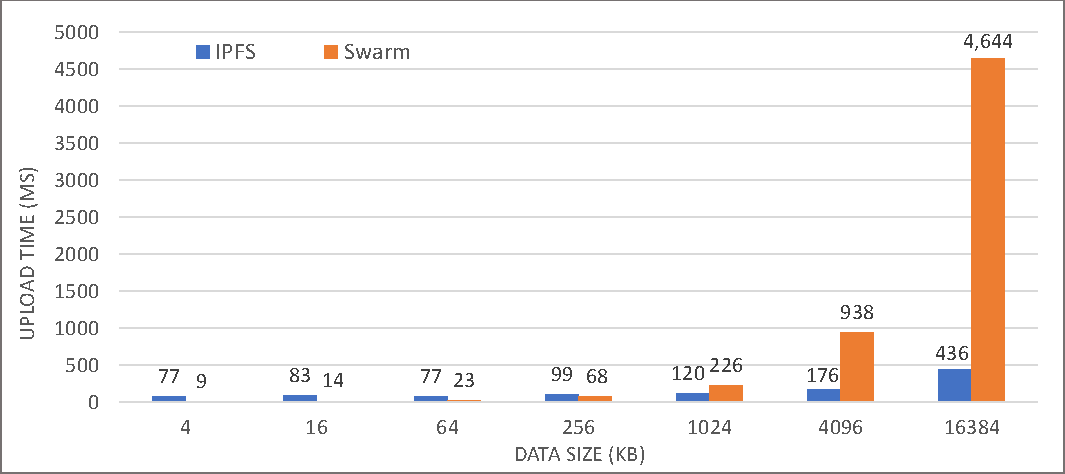
\includegraphics[width=\textwidth]{figs/ipfs_swarm_upload.pdf}}
\caption{IPFS-Swarm upload latency.}
\label{fig: ipfs_swarm_upload}
\end{figure}
\setlength{\belowcaptionskip}{-10pt}

As we can observe from Fig.~\ref{fig: ipfs_swarm_retrieve}, Swarm lacks in performance when it comes to retrieving data from local storage. That is due to the fact that all chunks split during the upload process must be individually fetched in order to reconstruct the original data. A large number of chunks implies a complex Merkle-Tree or Merkle-DAG. Thus, longer paths have to be resolved until each chunk is found, leading to greater retrieval time. Once again, it is clear that the chunk-size utilized within each platform’s architecture is a determining factor for their performance.

\begin{figure}[htbp]
\centerline{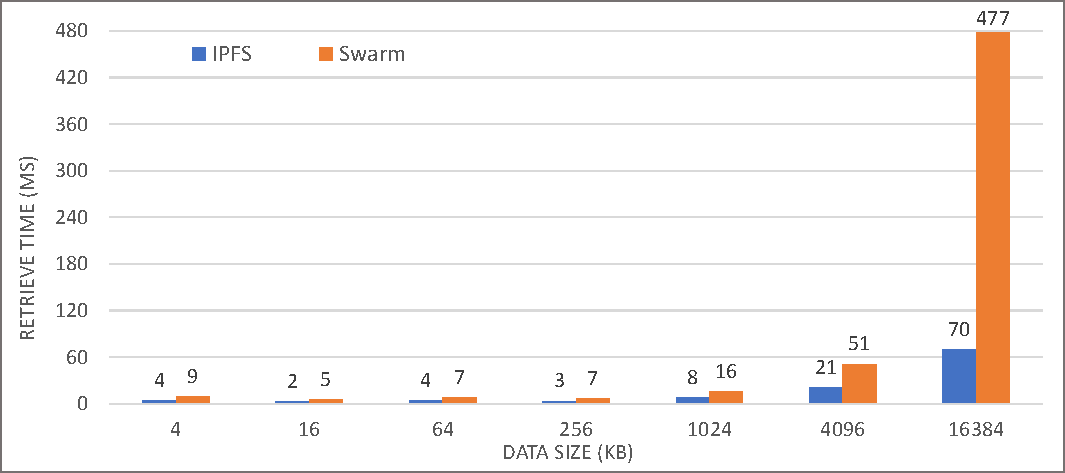
\includegraphics[width=\textwidth]{figs/ipfs_swarm_retrieve.pdf}}
\caption{IPFS-Swarm retrieval latency.}
\label{fig: ipfs_swarm_retrieve}
\end{figure}
\setlength{\belowcaptionskip}{-10pt}

We ought to clarify that by conducting these experiments we meant to compare the performance of IPFS and Swarm, regarding local upload and retrieval. The results are nothing but representative of how these platforms behave when exchanging data between remote nodes. Besides that, Swarm updated its networking protocol from devp2p to libp2p and introduced a new client, which we used during our experiments. The fact that it is in primary stage and improvements are frequently made might render our results obsolete in the near future.
\subsection{Remote Retrieval Performance}\label{subsection:evaluation_remote}
% TODO: review and remove comments

% \paragraph{Evaluated Scenarios}\label{subsection:remote_experiment_setup}
% In this subsection we evaluate the remote retrieval performance of IPFS and Swarm. With the term \textit{remote retrieval} we refer to the process of retrieving data that is not stored in the node's local storage and therefore needs to be fetched from the network. 

% First, we outline the set of experiments that we conducted. Then we present and discuss the results that we collected during our experiments. As part of this discussion, we draw conclusions about which platform performs better under the experimental environment we created.
% The simulated scenarios intend to cover a wide range of real-world situations that a user may encounter when retrieving content from platforms such as IPFS and Swarm. For instance, there desired data is immediately accessible from a directly connected peer. Alternatively, it might be cached by a nearby node other than the original uploader, thereby eliminating the need for a complete DHT query. 
To evaluate the retireval performance of IPFS and Swarm we simulate a wide range of real-world situations that a user may encounter when retrieving content from these platforms. For instance, the requested data is immediately accessible from a directly connected peer. Alternatively, it might be cached by a nearby node other than the original uploader, thereby eliminating the need for a complete DHT query. 

% In brief, we utilized our experimental setup to simulate the following four different scenarios:
We study the following four different scenarios:

\begin{itemize}[itemsep=0pt]
    \item  \textbf{simple}: For each round one node uploads a series of content, which is then downloaded by the remaining nodes. Given that the content is replicated amongst the nodes that download it, all nodes - except from the first one - that download it could potentially retrieve the content from a node other than the original uploader in case of IPFS or responsible storer nodes in the context of swarm.
    \item \textbf{no-cache}: For each round one node uploads a series of content and the rest of the nodes download it. Each downloader, after getting the content removes it from local storage. Regarding IPFS, this ensures that content is always retrieved from the uploader. In case of Swarm it ensures that the content isn't cached and therefore cannot be provided by the nodes that have already downloaded it.
    \item  \textbf{disconnect}: For each round, a single node uploads a series of content and the remaining nodes download it. Since the connection with the uploader isn't terminated instantly, the downloader - upon successfully retrieving the content - disconnects from the peer (uploader) from which the content was obtained. 
    \item \textbf{no-cache-disconnect}: Similar procedure to \textit{no-cache}, but the downloader - upon successfully retrieving the content - disconnects from the peer from which the content was obtained. Regarding IPFS, this ensures that content is always retrieved from the uploader and the nodes. In case of Swarm it ensures that the content isn't cached and therefore cannot be provided by the nodes that have already downloaded it.
\end{itemize}

% These scenarios were designed to cover most of the realistic cases a user might experience while retrieving content from a platform like IPFS ans Swarm. For instance, sometimes the requested data might be available in a direct peer and be fetched immediately. In other cases, a nearby node other than the uploader might have cached the data thus returning it back. 

We tested these cases repeatedly in multi-round experiments as discussed in the experimental setup section \ref{sec:setup_remote}
The corresponding results can either be presented as a total to give an overview of the interaction with IPFS and Swarm, or separately for each scenario.
%  \hl{...} 
% Our third dataset focuses on benchmarking content publication and retrieval performance. We use six virtual machines in six different regions on AWS. Namely, the t2.small machines run in me_south_1 (Bahrain), ap_southeast_2 (Sydney), af_south_1 (Cape Town), us_west_1 (N. California), eu_central_1 (Frankfurt) and sa_east_1 (São Paulo). On each machine we run a go-ipfs v0.10.0 instance acting as a DHT server node. We use these controlled instances to interact with the public IPFS network and per form tailored performance experiments

% Upon each iteration, a single node announces a new 0.5MB object (i.e., CID) to the network. Following this, all other nodes retrieve the object. This involves looking up the provider and peer records, connecting to the providing peer and then downloading the object. As soon as all remaining nodes have completed this process, they disconnect to prevent the next retrieval operation being resolved through Bitswap and instead resort to the DHT for lookup and discovery. It is worth noting that this is the closest one can get to a controlled experiment in the public IPFS network. This is because it

\begin{table}[H]
\centering
\begin{small}
\caption{Accumulated measurements for IPFS. The dataset consists of 3990 samples in total (including failures), with retrieval failure ratio of $\sim 30\%$ }
\label{tab:ipfs_all}
\begin{tabular}{@{}lccccccc@{}}
\toprule
Size & Mean & Median & IQR & Skewness & Min & Max & Sample Size \\ \midrule
4KB & 876.96 & 177.07 & 226.28 & 7.06 & 6.99 & 29391.19 & 415\\
16KB & 691.94 & 148.4 & 128.63 & 7.82 & 3.13 & 29803.37 & 390\\
64KB & 1031.23 & 215.52 & 251.2 & 6.47 & 3.32 & 29352.31 & 384\\
256KB & 751.66 & 273.82 & 362.55 & 10.53 & 38.86 & 30001.96 & 400\\
1MB & 959.27 & 315.87 & 1393.61 & 8.88 & 9.67 & 27258.05 & 410\\
4MB & 1126.27 & 449.5 & 942.13 & 7.03 & 99.65 & 27082.3 & 412\\
16MB & 1807.24 & 1271.9 & 1606.68 & 5.29 & 297.5 & 26714.33 & 398\\
\bottomrule
\end{tabular}
\end{small}
\end{table}

\begin{table}[H]
\centering
\begin{small}
\caption{Accumulated measurements for Swarm. The dataset consists of 2795 samples in total (including failures), with retrieval failure ratio of $\sim 8.5\%$ }
\label{tab:swarm_all}
\begin{tabular}{@{}lccccccc@{}}
\toprule
Size & Mean & Median & IQR & Skewness & Min & Max & Sample Size \\ \midrule
4KB & 67.32 & 52.38 & 72.62 & 2.06 & 1.19 & 420.3 & 395\\
16KB & 226.24 & 202.78 & 225.53 & 0.78 & 2.66 & 794.08 & 395\\
64KB & 352.05 & 321.35 & 185.17 & 0.94 & 3.32 & 1194.75 & 395\\
256KB & 506.17 & 469.51 & 248.64 & 0.71 & 4.69 & 1484.6 & 395\\
1MB & 1262.27 & 1211.74 & 512.95 & 0.07 & 10.56 & 2673.54 & 400\\
4MB & 3538 & 3497.82 & 1191.13 -& 0.59 & 34.05 & 7884.58 & 404\\
16MB & 9555.86 & 9047.49 & 2609.57 & 1.83 & 5822.69 & 20503.51 & 169\\
\bottomrule
\end{tabular}
\end{small}
\end{table}


% In your case, if outliers represent extreme performance instances (e.g., extremely fast or slow retrieval times) that are not representative of typical performance, it may be appropriate to remove them. Reporting metrics both before and after this process allows you to demonstrate the impact of this decision and to provide a more accurate representation of general performance patterns.
Tables \ref{tab:ipfs_all} and \ref{tab:swarm_all} are snapshots of the overall retrieval latency encountered during the experiments we conducted. The minimum and maximum values observed represent extreme performance instances (e.g., extremely fast or slow retrieval times) that are not representative of typical performance. In IPFS such low latency suggests that content is fetched from a directly connected peer using the Bitswap protocol, rather than through a DHT query. Conversely, our Swarm nodes may have already cached the content, if they were part of the forwarding path from the uploader to the neighborhood of responsibility. Latency in this cases, aligns with the local retrieval performance we discussed in section \ref{subsection:evaluation_local}

In addition, the measurements that we obtained are greatly skewed towards higher latency levels and demonstrate a substantial degree of dispersion, as indicated by the Skewness and IQR metrics. For a better comprehension of the particular data set's distribution, refer to Appendix A.
% TODO: add reference
%  \ref{chapter:appendix}. 

Most of the datasets we compiled  exhibit similar distributions, especially those regarding IPFS. In view of this, we applied the Inter Quartile Range formula to detect and remove outliers in all data sets. We opted for this method as it is better suited for skewed data with and isn't affected by outliers \citep{whaley_2005}. Part of the processed measurements is included in Appendix A. Upon examining the cleansed results, we conclude that the median even prior to removing the outliers is a reliable measure of central tendency.  Consequently, we refer to the median of the original measurements throughout this section.

The results we gather indicate that the chunk-size utilized within each platform’s architecture is a determining factor for their performance. As the size of the data increases, performance deteriorates substantially. Overall, for small data up to 4KB (one swarm-chunk) Swarm is notably more efficient. Then both platforms perform equally for data of 256KB or lower, but above this IPFS outperforms its counterpart.

However, it's important to take into account that large content in Swarm is fetched from multiple different nodes, potentially hundreds, that need to be discovered separately. The fact that even for 16MB data it takes about nine seconds for a complete retrieval and reconstruction, implies that Swarm's DISC model and routing approach is indeed effective. In a similar scenario, case IPFS requires approximately 1.2 seconds to locate a single node, establish a connection (if not already present) and retrieve the content. So, in cases where a large data set that consists of numerous chunks not hosted by a single node, PFS might actually exhibit slower performance compared to Swarm. 

% The measurements presented in Fig. 4.11, indicate that uploading data up to 256KB in Swarm is quite fast. Above this threshold, performance deteriorates substantially. We must consider that data are split into chunks which are hashed and organized in a Binary Merkle Tree. Obviously, the number of calculations included in this process is proportional to the size of the data and definitely affects the upload-time. IPFS behaves similarly, except that the size of the data has smaller impact on its

% performance. This mostly stems from the fact that chunk’s default size (256KB) in IPFS is 64 times the size of a Swarm chunk (4KB), rendering the process of splitting the data and organizing the chunks in a Merkle-Dag faster. Accordingly, the quite
% stable measurements for data up to 256KB are justified, as they fit in one chunk.

\begin{table}[H]
\centering
\caption{Accumulated measurements for the hosts participating in the experiments (IPFS).}
\label{tab:hosts_ipfs}
\resizebox{\textwidth}{!}{%
\begin{tabular}{@{}lcccccccc@{}}
\toprule
Host    & \multicolumn{7}{c}{Data Size}          & Failures (\%) \\ \midrule
& 4kb  & 16kb  & 64kb  & 256kb  & 1mb  & 4mb  & 16mb              \\ \midrule
degroot & 242.18 & 170.23 & 249.04 & 313.59 & 385.42 & 516.34 & 1499.17 & 6.5 \\
nancy & 144.66 & 140.35 & 153.46 & 155.1 & 306.77 & 376.46 & 1095.44 & 21 \\
lille  & 130.76 & 123.73 & 175.87 & 201.17 & 272.27 & 464.68 & 1098.98 & 44 \\
grenoble  & 143.28 & 142.05 & 157.99 & 168.82 & 304.62 & 389.84 & 997.39 & 36 \\
rennes  & 147.11 & 134.58 & 151.39 & 166.05 & 198.18 & 409.78 & 944.75 & 31 \\
sophia  & 159.15 & 153.47 & 198.03 & 216.53 & 243.13 & 449.6 & 1331.35 & 38 \\
\bottomrule
\end{tabular}
}
\end{table}


\begin{table}[H]
\centering
\caption{Accumulated measurements for the hosts participating in the experiments (Swarm).}
\label{tab:hosts_swarm}
\resizebox{\textwidth}{!}{%
\begin{tabular}{@{}lcccccccc@{}}
\toprule
Host    & \multicolumn{7}{c}{Data Size}          & Failures (\%) \\ \midrule
& 4kb  & 16kb  & 64kb  & 256kb  & 1mb  & 4mb  & 16mb              \\ \midrule
degroot & 106.78 & 356.69 & 455.06 & 659.04 & 1718.43 & 4606.77 & 11706.08 & 9 \\
nancy & 50.22 & 121.62 & 302.14 & 422.94 & 1141.65 & 3220.77 & 7399.17 & 9 \\
lille  & 31.63 & 62.44 & 267.23 & 365.31 & 976.45 & 2855.04 & 8544.81 & 8 \\
grenoble  & 52.5 & 185.15 & 312.46 & 476.18 & 1183.72 & 3485.26 & 9405.18 & 8 \\
rennes  & 53.18 & 129.48 & 313.64 & 439.33 & 1056.81 & 3412.36 & 8631.65 & 8 \\
sophia  & 62.76 & 266.15 & 339.32 & 510.98 & 1244.26 & 3528.51 & 9677.73 & 9 \\
\bottomrule
\end{tabular}
}
\end{table}

Consulting table \ref{tab:hosts_ipfs}, we deduce that our machine (degroot) requires more time to retrieve the data from the remaining hosts. This is expected if we take into account the topology described in section \ref{sec:setup_remote}. The node running in our machine always needs to interact with nodes located in france. On the contrary, nodes within the Grid5000 download a series of content from our node in Greece only in one round of each experiment. The distance of the physical underlying connection in the former case impacts IPFS's retrieval performance.

% The same applies to swarm,

The geographical distribution of nodes is also an important factor in Swarm, but it influences performance differently than in IPFS. It is not the topology that we created that affects performance, but the geographical location of the peers we are connected to and the overall topology of the testnet where we perform the experiments. 

Please note that content may be uploaded by our nodes, but is then distributed evenly across nodes in the network, which in turn serve it.
% stored and served by nodes that are evenly spread in the network.
% uniformly distributed in the overlay address space
% , i.e. evenly  
However, as we can see in fig \ref{fig:swarm_peers}, our node isn't connected to any peers in close proximity. Most of its peers are located in central and northern regions of Europe. Thus, for each download request a lond distance connection must be established, justifying the inferior performance of our machine reflected in table \ref{tab:hosts_swarm}.

% Hence, the geographical distribution of nodes in such networks contributes to performance, mainly due to the distance of the physical underlying connections.

% As a result of uniformity, a random set of chunked content will generate addresses evenly spread in the address space, i.e. imposing storage requirements balanced among nodes.
% Assuming any sample of base accounts independently selected, the resulting overlay addresses are expected to have a uniform distribution in the address space of 256-bit integers
% chunks are stored with nodes close to their address, fair and equal load balancing requires that the addresses of chunks should also be uniformly distributed in the address space, and have their content limited and roughly uniform in size.

\begin{figure}[htbp]
\centerline{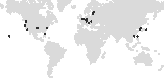
\includegraphics[width=\textwidth]{figs/swarm_peers.pdf}}
\caption{Peers of our Swarm node hosted in our machine.}
\label{fig:swarm_peers}
\end{figure}

Moreover, based on table \ref{tab:hosts_ipfs} we can infer that all hosts we established within Grid5000 experience frequent retrieval failures. Approximately 30\% - 40\% of the retrieval requests are unsuccessful, despite implementing a re-try mechanism to avoid such phenomenons (by default clients make three download attempts before aborting). This implies a connectivity issue, possibly due to the Grid5000's closed network, which hinders peer communication among the IPFS nodes we set up. Nodes inside Grid5000 are mostly visible to the outside world, as suggested by the low failure ratio of our machine, yet less visible to each other.

Networking issues were also encountered with the server-client system we developed. During the experiments, the clients running within the Grid5000 platform occasionally lost connection with the server (hosted in degroot), for a short period of time, after which they reconnected. To compensate for this, we developed a caching mechanism that enabled the server to coordinate the experiments effectively in case of reconnections or even if an experiment is terminated and restarted at a later time.

Unfortunately, even though certain measures were taken, such as increasing the retrieval timeout as much as 90 seconds and the retry parameter to 5, we were unable to resolve the connectivity issues in the IPFS-related experiments. However, in order to confirm our suspicions we performed the same experiments using our machine, an older machine we possess, and one host in Grid5000. Indeed, our machines demonstrate better retrieval success ratios (see table \ref{tab:miletus_degroot_nancy}).

The issue we've outlined might lower, to some extent, the overall quality of our measurements but yielded a valuable insight. That is, Swarm provides a more robust infrastructure that is resilient to networking issues. As observed in table \ref{tab:hosts_swarm}, the success ratio of retrievals in Swarm is higher. It seems that the content replication facilitated by the DISC storage model and  the consistency of the replication ensured by the pull-sync protocol even in high churn situations (refer to section \ref{subsection:swarm} for details) contribute to its more stable performance. 

In addition to that, Swarm's routing approach to relay requests from source to destination via peers that retain an open connection (direct peers) and then returning the response backwards through the same path, also alleviates connectivity issues. That is because the requestor only need to interact with a single peer, with whom it is already connected.

% \begin{figure}[htbp]
% \centerline{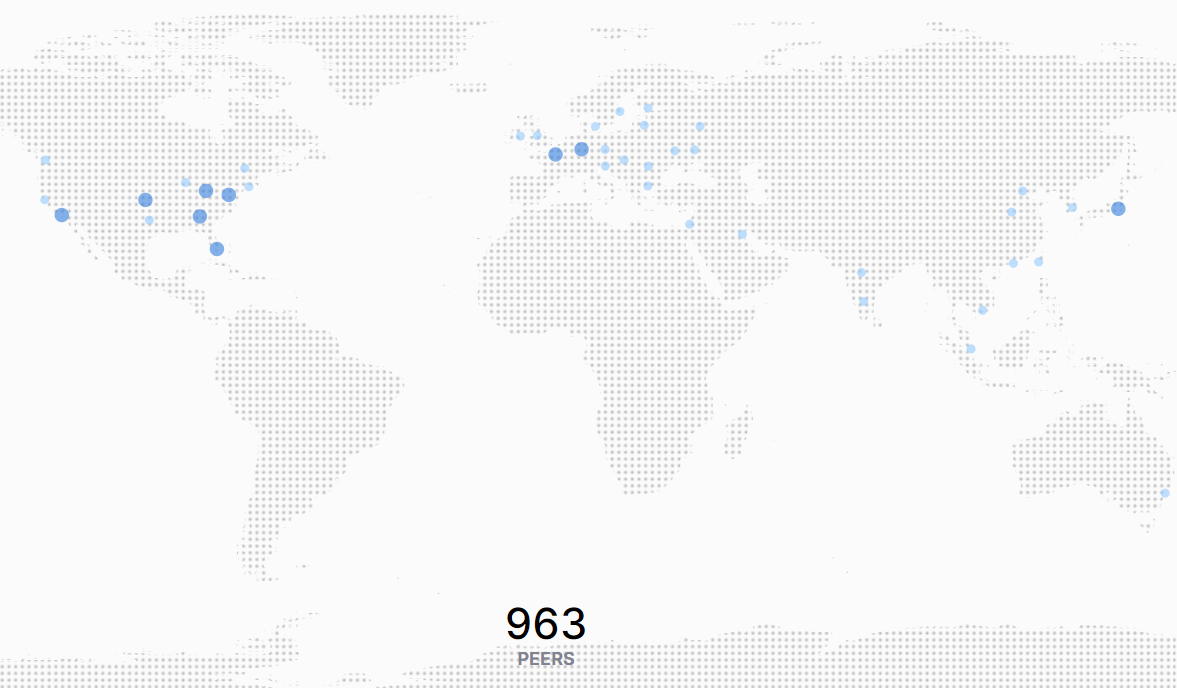
\includegraphics[width=\textwidth]{figs/ipfs_peers.png}}
% \caption{EIP standardization process.}
% \label{fig:ipfs_peers}
% \end{figure}

% \begin{table}[H]
% \centering
% \begin{small}
% \caption{Accumulated measurements for experiment \textit{simple} in IPFS. The dataset consists of 1050 samples in total (including failures), with retrieval failure ratio of $\sim 4\%$ }
% \label{tab:normal}
% \begin{tabular}{@{}lccccccc@{}}
% \toprule
% Size & Mean & Median & IQR & Skewness & Min & Max & Sample Size \\ \midrule
% 4KB & 472.96 & 211.66 & 109.01 & 3.69 & 30.04 & 5408.44 & 140\\
% 16KB & 135.24 & 150.64 & 28.92 & -1.06 & 30.90 & 203.29 & 143\\
% 64KB & 176.44 & 175.63 & 90.05 & -0.19 & 34.75 & 382.46 & 143\\
% 256KB & 247.11 & 239.92 & 161.51 & 1.17 & 38.85 & 712.93 & 145\\
% 1MB & 514.83 & 234.93 & 202.04 & 11.63 & 52.27 & 27258.04 & 146\\
% 4MB & 635.02 & 431.22 & 246.71 & 2.64 & 103.36 & 3260.39 & 145\\
% 16MB & 1797.22 & 1306.89 & 688.50 & 2.70 & 338.36 & 9525.16 & 144\\
% \bottomrule
% \end{tabular}
% \end{small}
% \end{table}


\begin{table}[H]
\centering
\caption{Accumulated measurements for each experiment in IPFS.}
\label{tab:experiments_ipfs}
\resizebox{\textwidth}{!}{%
\begin{tabular}{@{}lcccccccc@{}}
\toprule
Experiment    & \multicolumn{7}{c}{Data Size}          & Failures (\%) \\ \midrule
& 4kb  & 16kb  & 64kb  & 256kb  & 1mb  & 4mb  & 16mb              \\ \midrule
simple &  211.67 & 150.65 & 175.64 & 239.92 & 234.94 & 431.22 & 1306.9 & 4 \\
no-cache  & 218.6 & 123.72 & 72.86 & 97.88 & 116.75 & 198.57 & 638.54 & 24 \\
disconnect  & 144.2 & 139.67 & 1264.5 & 335.85 & 1360.46 & 494.24 & 1363.14 & 37 \\
no-cache-disconnect  & 159.82 & 180.53 & 266.43 & 375.63 & 1758.96 & 1114.13 & 1805.09 & 53 \\
\bottomrule
\end{tabular}
}
\end{table}

\begin{table}[H]
\centering
\caption{Accumulated measurements for each experiment in Swarm.}
\label{tab:experiments_swarm}
\resizebox{\textwidth}{!}{%
\begin{tabular}{@{}lcccccccc@{}}
\toprule
Experiment    & \multicolumn{7}{c}{Data Size}          & Failures (\%) \\ \midrule
& 4kb  & 16kb  & 64kb  & 256kb  & 1mb  & 4mb  & 16mb              \\ \midrule
simple & 51.22 & 212.43 & 307.71 & 481.13 & 1135.82 & 3563.81 & 9936.54 & 9 \\
no-cache  & 50.5 & 258.35 & 312.94 & 505.05 & 1212.22 & 3431.22 & 8391.32 & 9 \\
disconnect  & 52.5 & 183.78 & 351.1 & 467.8 & 1261.19 & 3507.51 & 8713.88 & 7 \\
no-cache-disconnect  & 53.43 & 152.27 & 328.79 & 447.65 & 1218.1 & 3514.01 & 8567 & 10 \\
\bottomrule
\end{tabular}
}
\end{table}


The measurements for IPFS and Swarm regarding the simulated scenarios we outlined in the begging of this section, have been accumulated in tables \ref{tab:experiments_ipfs} and \ref{tab:experiments_swarm}, respectively. It is clear that retrieval performance as well as the failure ratio in Swarm is similar in all cases. This is expected as data uploaded to Swarm is stored and served by nodes that are responsible for it. Therefore, preventing our nodes from caching the content or disconnecting from the original uploader has no affect in the ability of the storer nodes to provide the content. 
% The only thing we can ensure with the nodes we control..

On the contrary, in IPFS we observe great variability in the failure ratio throughout the experiments. In the first scenario where content can be downloaded either from the original uploader or from any of the remaining nodes that have already downloaded the content, most of the retrieval requests are successful. In the second scenario where it can be provided exclusively by the node that uploaded it, we see a drop in the success ratio. This suggests, that nodes within the Grid5000 exhibit better connectivity with our machine rather than among themselves. Simply put,  after a successful interaction with our machine, they register it as a peer, retain the connection and proceed to download content from it (instead of the original uploader) in the subsequent rounds. This phenomenon doesn't occur in the second scenario since our machine clears its cache, removing the data.

% However, \hl{as we discuss later in this section}, all nodes within the Grid5000 exhibit better connectivity with our machine rather than among themselves. So after a successful interaction with our machine, they register it as a peer, retain the connection and proceed to download content from it in the subsequent rounds. This phenomenon doesn't occur in the second scenario since our machine clears its cache, removing the data.

% These  findings suggest that \hl{within our experimental environment,} data retrieval is more successful from a direct peer that has cached the content, hence, the increased failures in the second case. Note that in both cases the connection with the uploader isn't forcibly ended and that all nodes interact at least once with each other. However, \hl{as we discuss later in this section}, all nodes within the Grid5000 exhibit better connectivity with our machine rather than amongs themselves. So after a successful interaction with our machine, they register it as a peer, retain the connection and proceed to download content from it in the subsequent rounds. This phenomenon doesn't occur in the second scenario since our machine clears its cache, removing the data.

The two remaining scenarios seem to adhere to the same rationale. Moreover, in every round, the downloader intentionally disconnect from the uploader, thus decreasing the set of potential peers that may have cached the content. 
% \hl{More importantly, they disconnect from our node when it acts as an uploader}. 
As a result, about 37\% and 53\% of the retrieval requests fail in the third and fourth scenarios, respectively.

% As for the retrieval latency, no exceptional divergence is observed. 
Earlier in this section, we mentioned our concerns about the results being affected by the connectivity issues we discussed. Thus we do not proceed to make any assumptions regarding the retrieval latency. The conclusion drawn from this set of results is that in a less-than-ideal connectivity environment like ours, the smaller the pool of potential content providers the more the retrieval process is impeded.

% by limiting the set of connected peers of 
% The only insight that the measurements provide is that the latency increases in parallel to the data size. Earlier in this section, we mentioned our concerns about the results so we will not proceed to make any assumptions.

% Specifically, all nodes within the Grid5000 seem to exhibit better connectivity with our machine rather than amongst themselves. Consequently, following a successful interaction with our machine, they register it as a peer, maintain the connection, and proceed to download content from it. This phenomenon doesn't occur in the second scenario since our machine (degroot) clears its cache, removing the data. This difference is discussed further in the following sections.

% In the first two scenarios, performance is slightly higher for 4kB, then drops and increases in parallel to the data size. Th


















